\section*{Introduction}
Exploration behavior can have two very different explanations depending on whether an animal might receive a reward. If there is no reason to expect a reward, exploration is treated as a search for information. For example, when a rat is placed in a novel environment it will explore even if no food and water is expected \cite{Berlyne1950}. We equate this with curiosity \cite{Berlyne1950,Schmidhuber1991,Kidd2015,Jaegle2019,Sumner2019,Wang2019,Auersperg2015}. If reward is expected however exploration is interpreted as a search for reward \cite{Gupta2006,Sutton2018,Woodgate2017,Lee2011a,Schulz2018a,Calhoun2014}.

An open problem in the decision sciences is to unify exploration with exploitation, which we define as the policy of choosing the most rewarding action. This union is known to be difficult and the conflict between them leads to the famous exploration-exploitation dilemma \citep{Kelly1956,Berger-Tal2014,Dayan1996,Thrun1992,Mehlhorn2015,Kobayashi2019}. We illustrate this classic paradox in Fig. \ref{fig:bee}a.

In this paper, we show that exploration is better handled by an information search, even when the goal is to collect the most reward. We can justify our use of curiosity because it is already known to be a primary drive in most, if not all, animals \cite{Berlyne1950,Loewenstein1994,Inglis2001}. It is as strong, if not sometimes stronger, than the drive for reward \cite{Loewenstein1994,Kidd2015,Gottlieb2018,Sumner2019,Gopnik2020,Song2019,Wang2019}. We illustrate our alternative in Fig. \ref{fig:bee}b.

\begin{figure}
	\begin{fullwidth}
	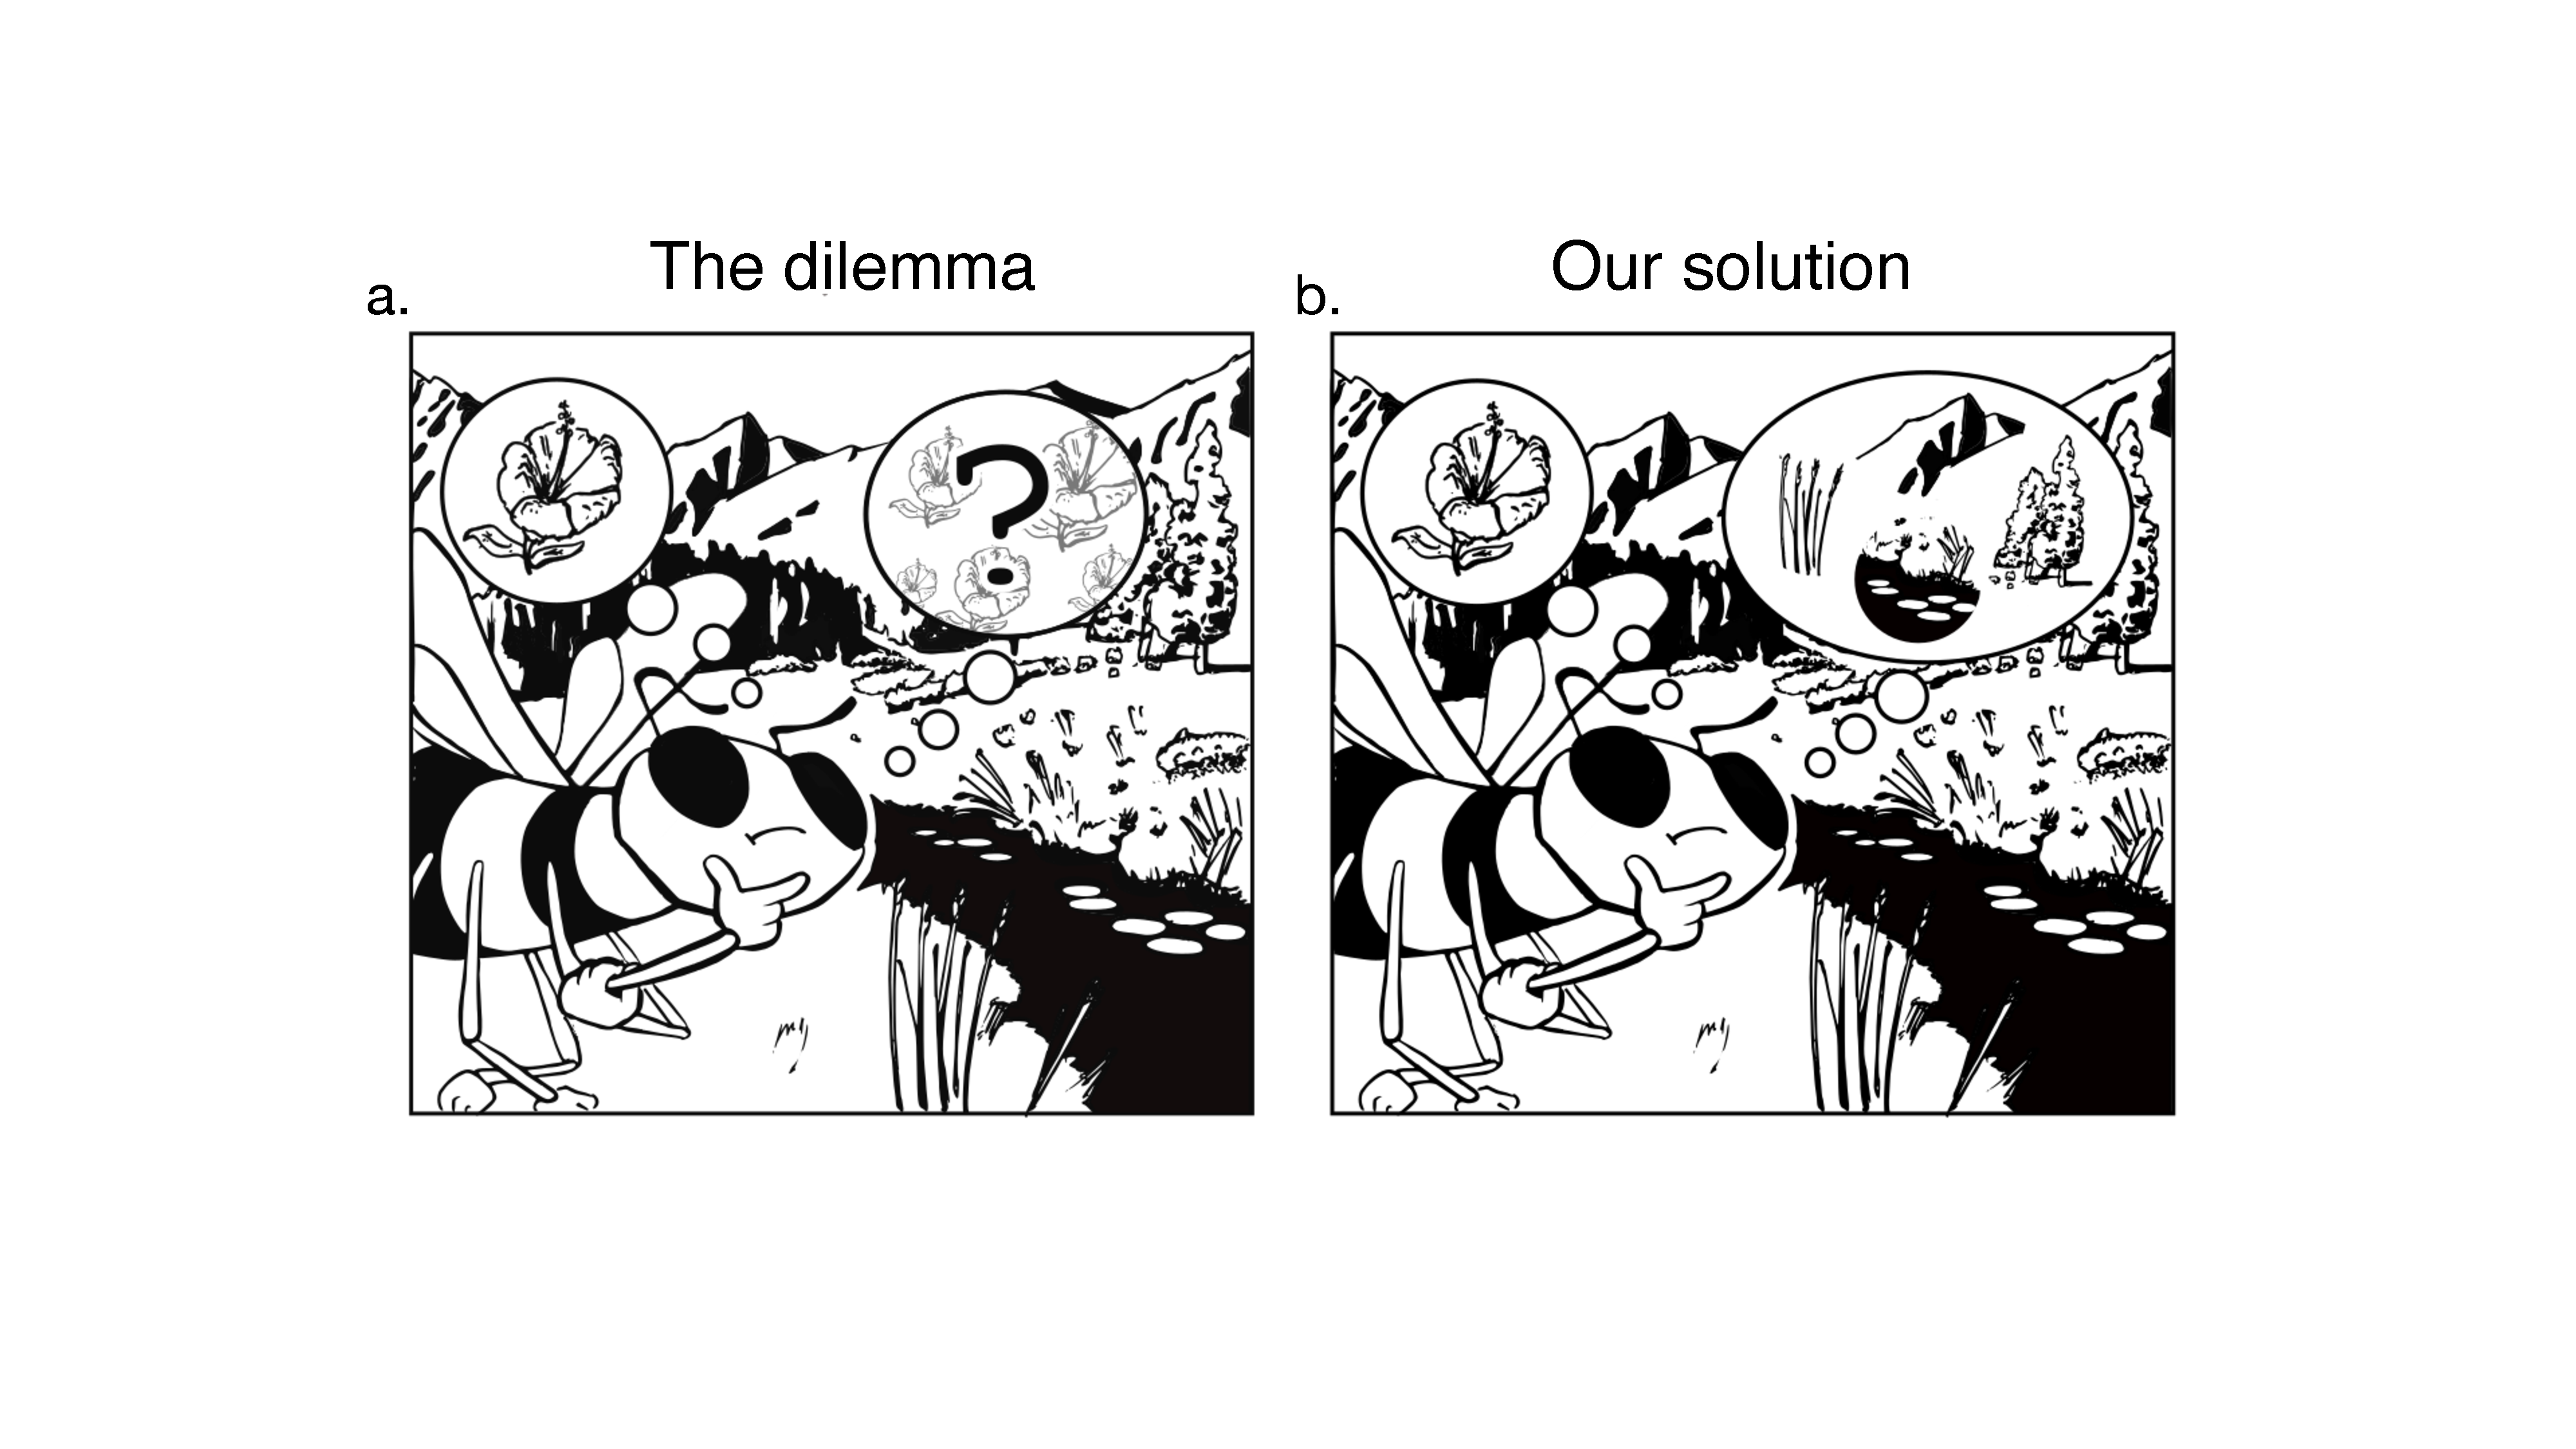
\includegraphics[width=.9\linewidth]{img/bee.pdf} 
	\caption{Two views of exploration and exploitation. \textbf{a}. The dilemma: either exploit an action with a known reward (e.g., return to the previous flower) or explore other actions on the chance they will return a better outcome. The central challenge here is that the outcome of exploration is uncertain, and filled with questions. \textbf{b}. An alternative view of the dilemma, with two goals: either maximize rewards \textit{or} maximize information value,s with a curious search of the environment. \textit{Artist credit}: Richard Grant.}
	\label{fig:bee} 
	\end{fullwidth}
\end{figure}

If exploration is just a search for information, then what was the dilemma can be divided into two problems. One problem is exploration (recast as a curious search). The other is exploitation, which still means a search for max reward. The focus of this paper is deriving a greedy and deterministic algorithm for solving both problems, simultaneously. We first develop a new mathematical view of information value, curiosity, and a new understanding of ideal curious search. The second half uses these first results to prove our curiosity trick leads to an optimal value solution for nearly all explore-exploit decisions.